\chapter{Project implementation}
\label{chapter5}
The solving methodology described will be applied to a specific test case.
%The project is developed in Pandapower a, Python based, power system analysis tool aimed at automation of static and quasi-static analysis and optimization of balanced power systems \cite{pandapower}.

%GYM-ANM on github, report branch 04/04/2022

\section{MV Oberrhein}
\label{sec:MVober}
%https://ietresearch.onlinelibrary.wiley.com/doi/epdf/10.1049/iet-gtd.2019.1602
The network used for these experiments is the MV Oberrhein network from Pandapower. MV Oberrhein is a real distribution located at Upper Rhine  (German:  Oberrhein),  Germany. This network is a generic 20 kV power system serviced by two 25 MVA HV/MV transformer stations. The network supplies 141 HV/MV substations and 6 MV loads through four MV feeders. The network layout is meshed, but the network is operated as a radial network with some open sectioning points, i.e., redundant lines/cables. This is common in real network: they are meshed but they operate in a radial way.\\
The grid also includes geographical information of lines and buses and is assembled from openly available data.  \\

A representation of the network can is presented in \ref{fig:MVober}. The blue dots represent the buses where load and/or generators are connected and the yellow squares represent the HV/MV substations.
\begin{figure}[H]
\centering
    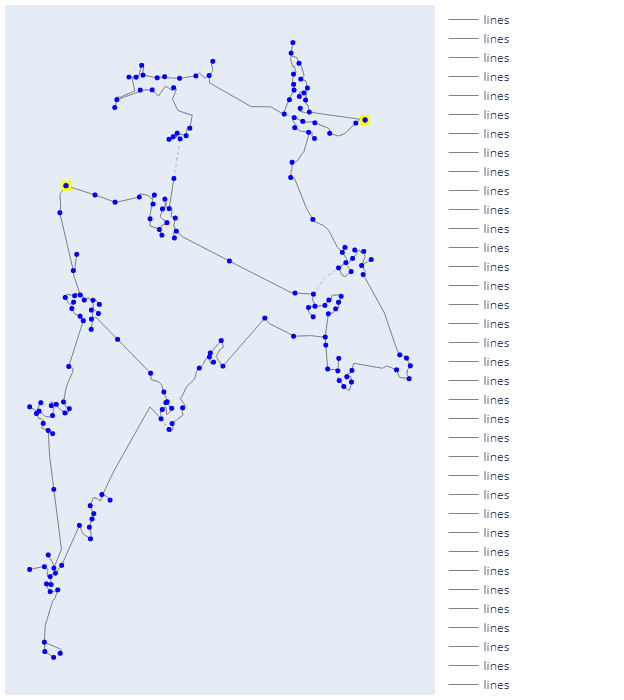
\includegraphics[width=.33\linewidth]{images/MVOberr/Full.png}
\caption{MV Oberrhein network. \emph{add feeders division(?)}}
\label{fig:MVober}
\end{figure}

To simplify the situation, the network can be divided in 2 independent parts [\href{https://kobra.uni-kassel.de/bitstream/handle/123456789/12005/kup_9783737608725.pdf?sequence=1&isAllowed=y}{ref}].

\begin{figure}[h]
\centering
    % 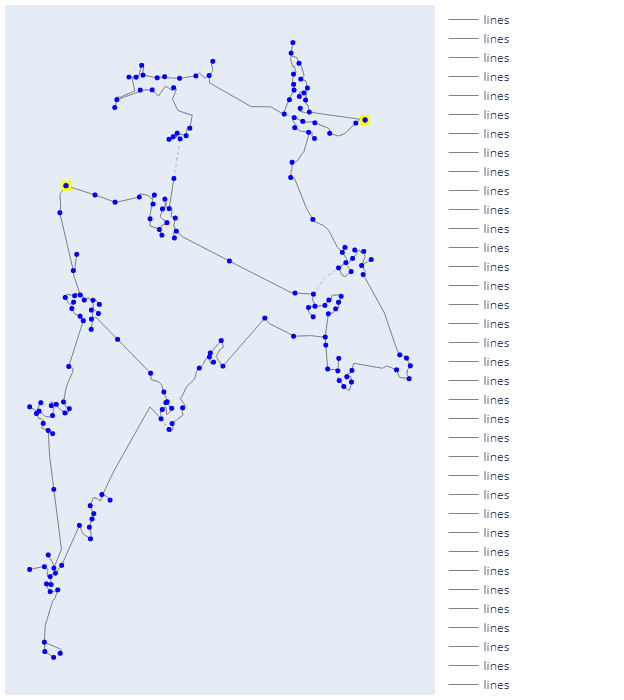
\includegraphics[height=0.33\linewidth,width=.32\linewidth]{images/MVOberr/Full.png}
    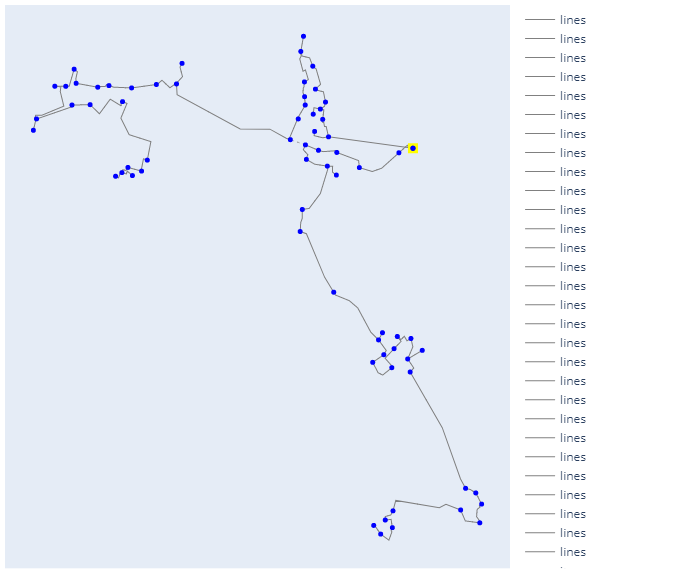
\includegraphics[height=0.33\linewidth,width=.32\linewidth]{images/MVOberr/Half1.png}
    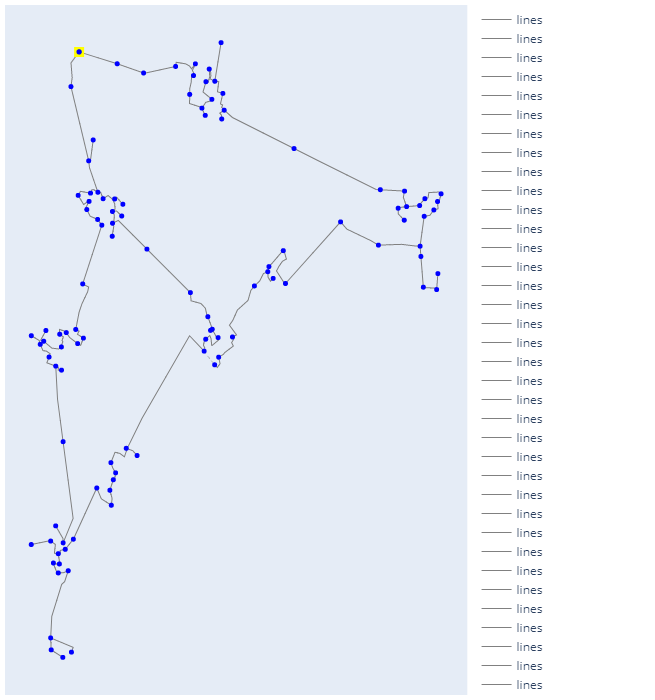
\includegraphics[height=0.33\linewidth,width=.32\linewidth]{images/MVOberr/Half2.png}
\caption{MV Oberrhein network. Used network: middle one \\
TODO add letters}
\label{fig:gym_anm_net}
\end{figure}

The model consist of: one external grid, one transformer, 70 buses, 61 loads and 60 renewable generators.

\subsection{Simbench database}
\label{simdata}
The time series dataset used is taken from the Simbench database. This database refers to some real distribution networks in Germany in the year 2016. SimBench includes multiple time series for one year with 15 min resolution for load, generation and storage units. All time series came as active and reactive power. The time series were grouped by element type, reducing the total number of required time series to a reasonable number, while retaining the possibility to model individual nominal power \cite{Simbenchds0}. All active power values are normalized to the maximum active power value.\\

Power utilities commonly use generic load profiles to group commercial customers with similar load shapes into categories or standard load profiles (\glspl{SLP}). \\
The most commonly used profiles set is developed by the German Association of Energy and Water Industries (\gls{BDEW}). It comprises eleven aggregated profiles, one for residential consumers (H0), three for agricultural (L0-L3), and seven for commercial consumers with different opening hours (G0-G6). They are differentiated into workdays, Saturdays and Sundays as well as three seasonal categories winter, summer, and transitional. The set also includes two profiles for street lightning (B0) and band load (G7). \\
The generation time series for photovoltaics (\glspl{PV}), wind energy and biomass generated for the SimBench dataset are created using the agent-based simulation tool for optimized grid expansion planning SIMONA. SIMONA's power plant models receive real weather data of Germany from the German Weather Service in 2011 for Wind and 2012 for \gls{PV} time series as input data. \\
For 2011 and 2012 generation data, the time axis is adjusted to 2016 by shifting days so that they correspond to the nearest weekday\cite{Simbenchds1}.\\

\begin{figure}[h]
\centering
    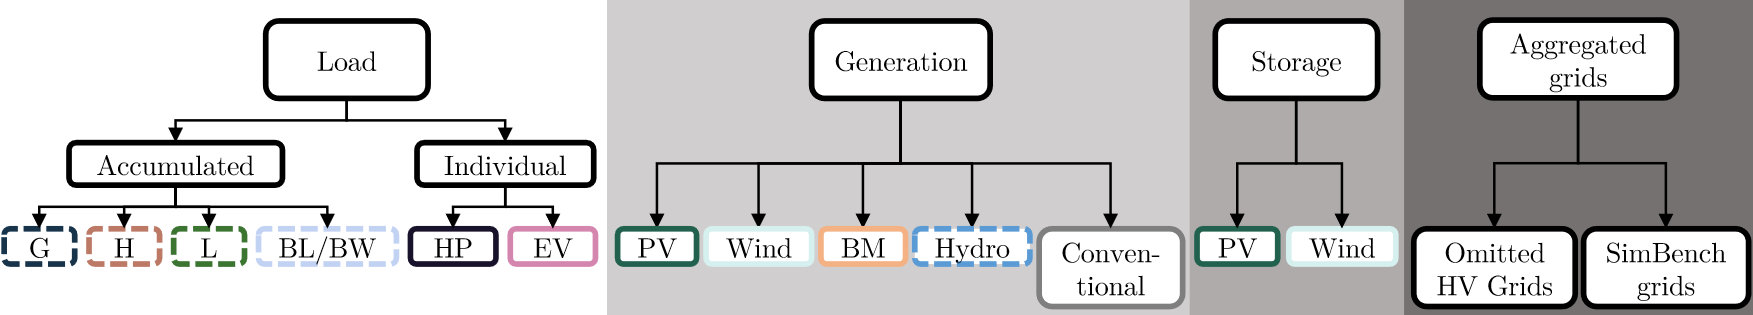
\includegraphics[width=.9\linewidth]{images/MVOberr/SimBench time series types.PNG}
\caption{Overview of the SimBench time series type}
\label{fig:SBtimeseriestype}
\end{figure}

The load time series were distinguished between real measured accumulated, highlighted with a dash, and simulated individual consumers, marked with a solid frame in Figure \ref{fig:SBtimeseriestype}. \\

\subsection{Time series}
\label{ts}
Some time series from the Simbench database are taken to adapt to the number of loads and \glspl{DER} of the MV Oberrhein network in consideration. \\

As said, each element (load or generator) falls under a specific profile type that represent the consumption or generation over time.

\begin{figure}[H]
\centering
    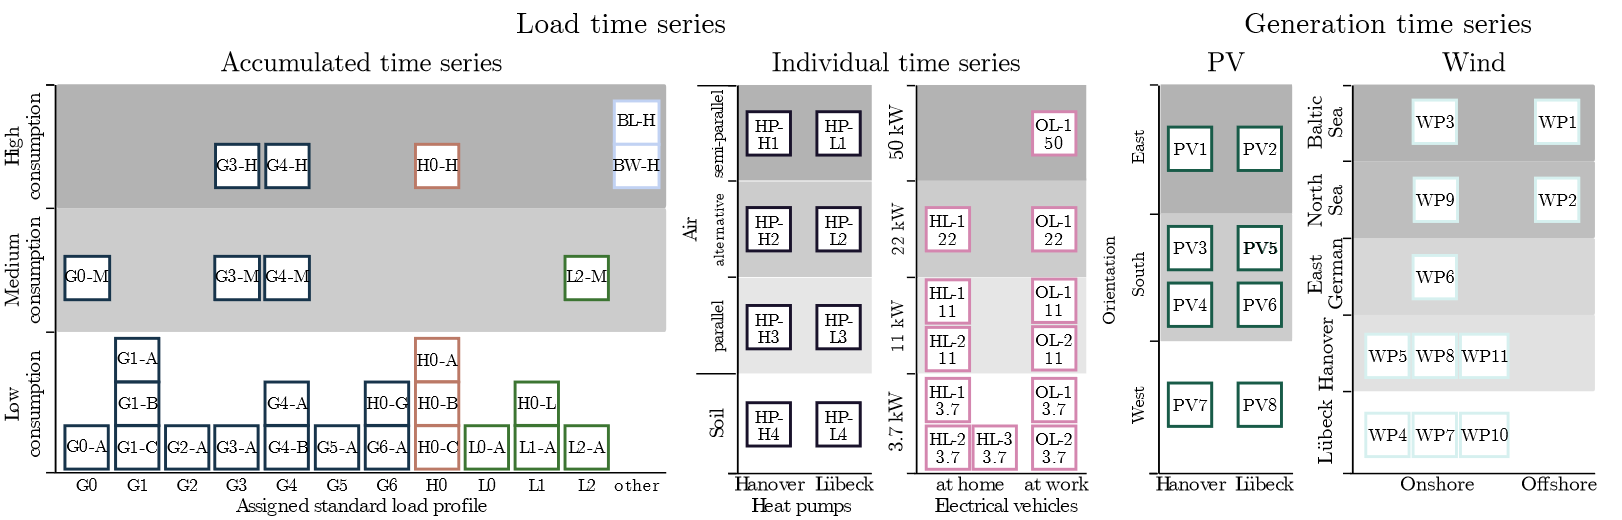
\includegraphics[width=.9\linewidth]{images/MVOberr/SimBench load and generation time series.PNG}
\caption{Load and generations profiles}
\label{fig:gym_anm_net}
\end{figure}

In this case, the profile's types for loads and \gls{DER} are chosen so that every profile type is present to have a network as close as possible to a real network. \\
The profiles' distribution in the Pandapower network is as follows:

\begin{algorithm}[h]
\State Load elements by type: \{{'G3-A': 2, 'H0-L': 3, 'G2-A': 5, 'G3-M': 2, 'G5-A': 2, 'L1-A': 3, 'L0-A': 2, 'H0-C': 6, 'H0-G': 3, 'G1-B': 2, 'G0-A': 4, 'L2-A': 2, 'L2-M': 3, 'G1-C': 2, 'G6-A': 3, 'G0-M': 3, 'G1-A': 3, 'G4-B': 2, 'H0-B': 3, 'G4-A': 3, 'H0-A': 3\}}
\State RES elements by type: \{'WP4': 6, 'PV5': 8, 'PV8': 8, 'PV1': 6, 'PV7': 6, 'PV3': 7, 'PV6': 6, 'PV4': 7, 'WP7': 6\}}
\end{algorithm}

\noindent where the letters stand for: commercial enterprises (G), households (H), agricultural holdings (L) and industrial companies (BL/BW)'; with last letters –A to C indicating low consumption, -M medium consumption, and -H high consumption customers. \\
For the \gsl{DES} device there are photovoltaics \glspl{PV} and wind parks \glspl{WP}. It is possible to notice a bigger presence of \glspl{PV} over \glspl{WP}.\\
% It is important to mention that the \gls{DES} devices are considered as static generators (sgen)

The loads and \glspl{DER} are chosen so that different profile types are present.

\begin{figure}[H]
\centering
    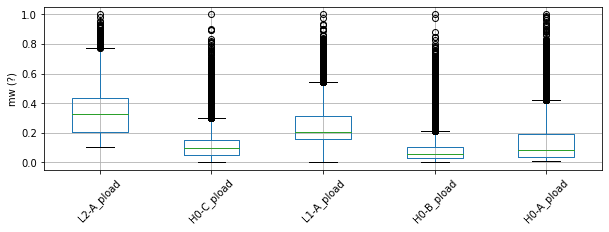
\includegraphics[width=.8\linewidth]{images/MVOberr/BoxPlotLoad.png}
    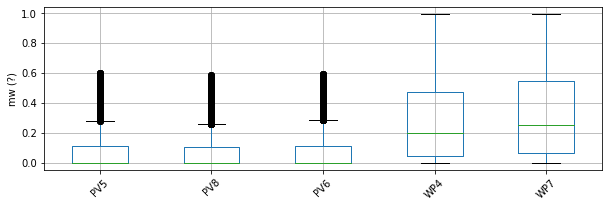
\includegraphics[width=.8\linewidth]{images/MVOberr/BoxPlotRes.png}
\caption{Box plots of load and generation for each profile type}
\label{fig:gym_anm_net}
\end{figure}

Since the profiles are similar for every element of the same type, some noise is added to increase randomness. In particular, the noise added is a scaling factor in the range [0.85,1.15]. The scaling factor allows avoiding negative values in case of a value lower than 1; subtraction may result in a negative value of reactive power for a particular load. \\

\subsection{Partial observability}
To simulate the partial observability problem, some time series are considered as unknown: for just some sparse time steps (missing values) or not available at all. \\

In particular, $x_1\%$ values are randomly selected and set as \emph{NAN} and $x_2\%$ time series of some devices are completely deleted.\\
\emph{Q: Any realistic value for $x_1$ and $x_2$? \label{q:partialobvals}} \\

\noindent These missing values are reconstructed as follows:
\begin{itemize}
    \item for the \emph{NAN} case, it is possible to fill the missing values with the preceding available value. This method, even if simple, is efficient for some reasons: the $\Delta t$ considered is not too large, so it is plausible to expect that loads and generators' values do not change rapidly; it is easy to compute with respect to more complex methods; using only past values allows not to wait for the future values, waiting for the future values may not be acceptable after a deployment of the model.
    
    \item For the case of time series not available at all, it is possible to use balancing flow techniques or generative models like for example \gls{GAN}.\\
    \emph{Q: in this case, isn't a bit overkilling using such method when the load and generator's profile are equal/similar? \label{q:gan}}
\end{itemize}

\subsection{Processing}
For this case, the information used to build the dataset is the voltage magnitude at each buses. The time series will be divided in windows of length, $h$ for the inputs $\textbf{x}$ and length $n$ for the outputs $\textbf{y}$. \\

It is possible to define $\textbf{x}$ as follows:

\begin{equation}
  \begin{aligned}
    \textbf{x}  = 
        \begin{bmatrix}
        V^1_{t-h+1} & V^1_{t-h+2} & \cdots & V^1_{t-1} & V^1_{t} \\
        & & & & \\
        
        V^2_{t-h+1} & V^2_{t-h+2} & \cdots & V^2_{t-1} & V^2_{t} \\
        & & & & \\
        
        \vdots & \vdots & \ddots & \vdots & \vdots \\
        & & & & \\
        
        V^{n-1}_{t-h+1} & V^{n-1}_{t-h+2} & \cdots & V^{n-1}_{t-1} & V^{n-1}_{t} \\
        & & & & \\
        
        V^n_{t-h+1} & V^n_{t-h+2} & \cdots & V^n_{t-1} & V^n_{t} \\
        \end{bmatrix}
  \end{aligned}
\end{equation}
\noindent where $V^i_t$ is the voltage level $V$ of bus $i$ at time stamp $t$. \\

\noindent Instead, $\textbf{y}$ can be defined as previously mentioned: 
\begin{equation}
    \begin{aligned}
        \textbf{y} = [C_{t+1},C_{t+2}, \dots, C_{t+n-1},C_{t+n}]
    \end{aligned}
\end{equation}
\noindent where $C_t$ is the condition of the system at time stamp $t$, with $C_t=1$ if the network is in a critical situation or $C_t=0$ if it is in a normal situation. \\

A time step is considered critical when the voltage of at least one of the buses is out of the boundaries $V_i < v^{\text{min}}$ (under voltage) or $V_i > v^{\text{max}}$ (over voltage), where $v^{\text{min}}$ is the minimum acceptable voltage, 0.95 \gls{pu}, and $v^{\text{max}}$ is the maximum one, 1.05 \gls{pu}.

% \subsection{Different cases}
% With a similar approach for adding some noise to the time series, it is possible to easily create different cases, changing the scaling factors.

% \begin{figure}[H]
% \centering
%     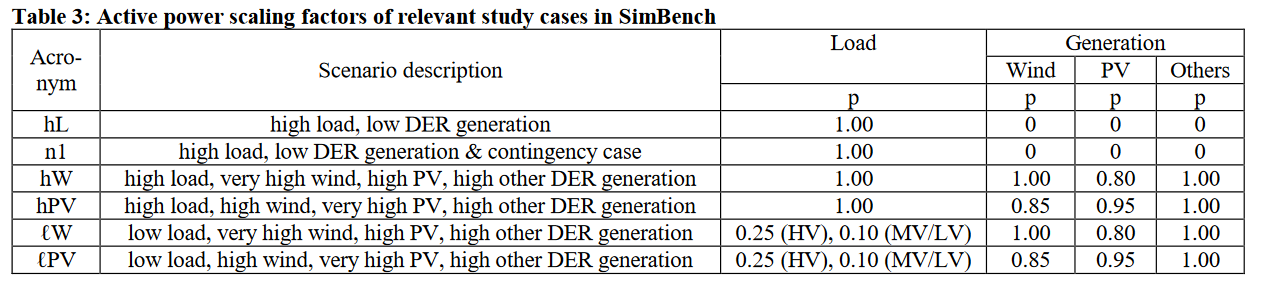
\includegraphics[width=.9\linewidth]{images/MVOberr/Cases.PNG}
% \caption{Possible cases. [\href{https://www.cired-repository.org/bitstream/handle/20.500.12455/526/CIRED \%202019 \%20- \%20139.pdf?sequence=1&isAllowed=y}{ref}] }
% \label{fig:gym_anm_net}
% \end{figure} 



% \begin{figure}[h]
% \centering
%     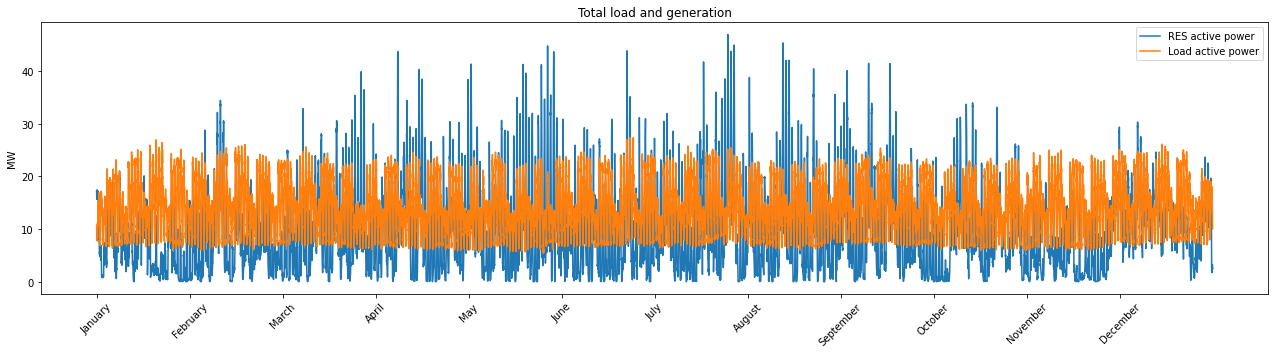
\includegraphics[width=.9\linewidth]{images/MVOberr/Load&Gens.png}
% \caption{Sum of load energy consumption and energy generation over the considered year}
% \label{fig:gym_anm_net}
% \end{figure}

% [old] It is possible to notice a higher consumption of energy over the production, especially at the beginning and end of the year, when the sun intensity is not too high. \\

% \subsubsection{Case: High generation}
\subsection{No partial-observability problem}
As mentioned the time series were normalized so it is possible to use some scaling factors to generate different case. The high generation case refers to scaling factors, as follows:
\begin{algorithm}[H]
    \State {scale\_factor\_load = 1} 
    
    \State {scale\_factor\_sgen = 1.5}
\end{algorithm}

These values are chosen to fit the load and generation profile with the peak capacity of the MV Oberrhein network.

\begin{figure}[H]
\centering
    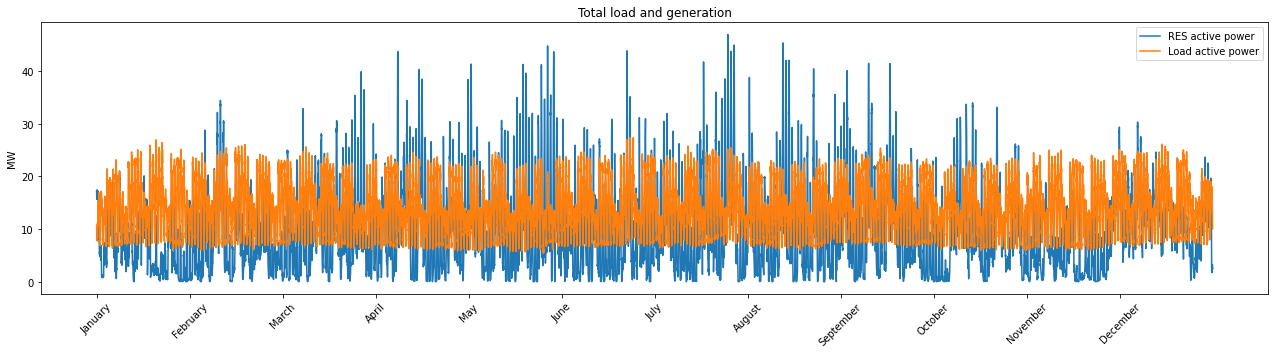
\includegraphics[width=.9\linewidth]{images/MVOberr/Load&Gens.png}
\caption{Sum of load energy consumption and energy generation over the considered year}
\label{fig:gym_anm_net}
\end{figure}

The consumption values are as a typical MV network (\cite{MVnetworks}), while the generation is higher. This case can represent a future power network when the number and the performance of \gls{DER} devices increase, so to have a generation of power higher than the demand; especially during the summer period when the consumption is lower and the generation is higher.\\
Such situation is critical for a network since the surplus energy increase the voltages at the buses that may experience problems or over voltages. \\

% \begin{figure}[h]
% \centering
%     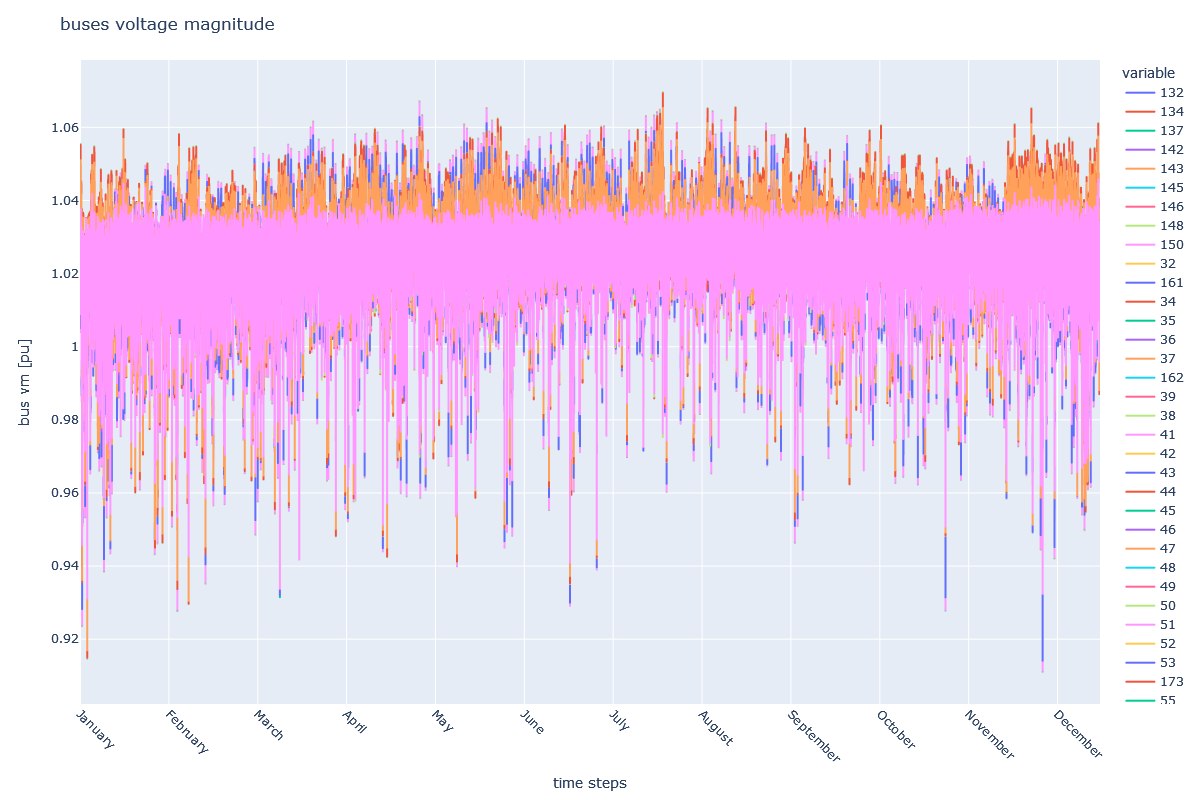
\includegraphics[width=.9\linewidth]{images/MVOberr/High gen.png}
% \caption{Case high generation. Voltage buses results obtained running the time series}
% \label{fig:gym_anm_net}
% \end{figure}

To test whether an over voltage situation occurs or not, the \gls{PF} is calculated using the Pandapower solver.\\
It is possible to see that there are some overvoltage problems. \\
The problems are highlighted in the following plot.

\begin{figure}[H]
\centering
    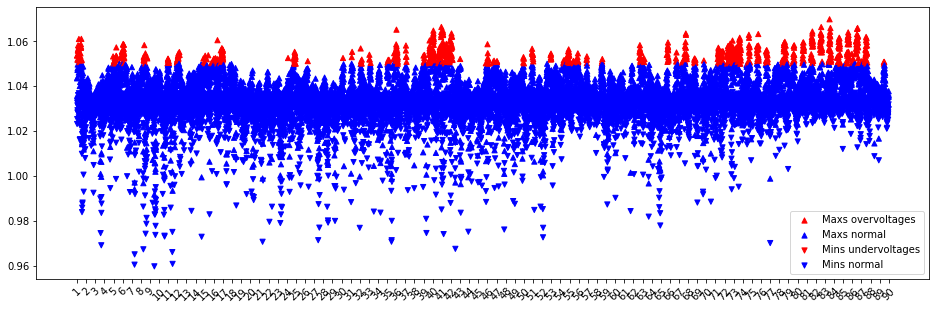
\includegraphics[width=.8\linewidth]{images/MVOberr/CriticalSituation.png}
\caption{In this plot, the maximum and minimum values found for each time step and plotted, so for each time step there are two values representing the highest and lowest value among each bus. The colours, blue and red, represent the normal or critical condition}

 \end{figure}

The full dataset is divided in train, validation and test set with the following proportions: 0.7, 0.2, 0.1 respectively. \\

The dataset is highly imbalanced since the number of times the network is in a critical situation are lower than the number of times the network is under normal situation. This is what usually happens in a power system: networks perform well most of the time and the critical conditions are few.

\begin{algorithm}[H]
    \State Number of critical situations: 1284, over 35040 time steps, ratio: 3.7\% \emph{realistic?}
    \State Number of critical instants in Train set: 646, ratio: 2.6\%
    \State Number of critical instants in Val set: 193, ratio: 2.8\%
    \State Number of critical instants in Test set: 445, ratio: 12.7\%
\end{algorithm}

The data input shape is as follows:

\begin{algorithm}[H]
    \State Inputs shape (batch size, time steps, features): (512, 16, 69)
\end{algorithm}

Three main \gls{ANN} are tested:
\begin{itemize}
    \item \gls{MLP} with two hidden layers of size 192 and 64.
    \item \gls{CNN} with one convolutional layer and one dense layer with 128 neurons.
    \item \gls{RNN} with one \gls{LSTM} as recurrent unit and one dense layer with 128 neurons.
\end{itemize}
All models have as last output layer a fully connected layer whose output size is just one neuron with a Sigmoid activation function.\\

The test are perform considering a temporal window $h$ of 16 time steps (4 hours in the past), while the output window is just one time step in the future (\emph{can be changed to any number}):
\begin{algorithm}[H]
    \State Labels shape (batch size, time steps): (512, 1)
\end{algorithm}

% \begin{figure}[h]
% \centering
%     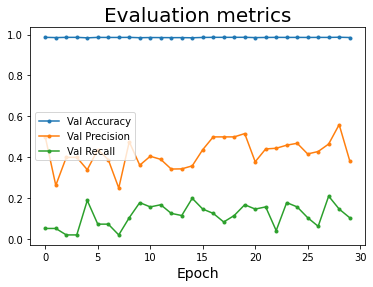
\includegraphics[width=.7\linewidth]{images/MVOberr/DenseNNResult.png}
% \caption{Training history on the validation set for the \gls{MLP} model}
%  \end{figure}

input |V|, h = 16 (4 h) \\
\begin{table}[H]
\centering
\begin{tabular}{l|l|l|l|}
\cline{2-4}
 & \begin{tabular}[c]{@{}l@{}}Test\\ Accuracy\end{tabular} & \begin{tabular}[c]{@{}l@{}}Test\\ Precision\end{tabular} & \begin{tabular}[c]{@{}l@{}}Test\\ Recall\end{tabular} \\ \hline
\multicolumn{1}{|l|}{MLP} & 0.92 & 0.83 & 0.45 \\ \hline
\multicolumn{1}{|l|}{CNN} & 0.89 & 0.55 & 0.93  \\ \hline
\multicolumn{1}{|l|}{RNN} & 0.87 & 0.64 & 0.98 \\ \hline
\end{tabular}
% \caption{}
\label{tab:my-table}
\end{table}


input |V|, h = 4 (1 h) \\
\begin{table}[H]
\centering
\begin{tabular}{l|l|l|l|}
\cline{2-4}
 & \begin{tabular}[c]{@{}l@{}}Test\\ Accuracy\end{tabular} & \begin{tabular}[c]{@{}l@{}}Test\\ Precision\end{tabular} & \begin{tabular}[c]{@{}l@{}}Test\\ Recall\end{tabular} \\ \hline
\multicolumn{1}{|l|}{MLP} & 0.94 & 0.72 & 0.93 \\ \hline
\multicolumn{1}{|l|}{CNN} & 0.90 & 0.56 & 0.99  \\ \hline
\multicolumn{1}{|l|}{RNN} & 0.95 & 0.76 & 0.94 \\ \hline
\end{tabular}
% \caption{}
\label{tab:my-table}
\end{table}



input RES p, h = 16 (4 h) \\
\begin{table}[H]
\centering
\begin{tabular}{l|l|l|l|}
\cline{2-4}
 & \begin{tabular}[c]{@{}l@{}}Test\\ Accuracy\end{tabular} & \begin{tabular}[c]{@{}l@{}}Test\\ Precision\end{tabular} & \begin{tabular}[c]{@{}l@{}}Test\\ Recall\end{tabular} \\ \hline
\multicolumn{1}{|l|}{MLP} & 0.87 & 0 & 0 \\ \hline
\multicolumn{1}{|l|}{CNN} & 0.87 & 0.49 & 0.47  \\ \hline
\multicolumn{1}{|l|}{RNN} & 0.87 & 0 & 0 \\ \hline
\end{tabular}
% \caption{}
\label{tab:my-table}
\end{table}


input RES p, h = 4 (1 h) \\
\begin{table}[H]
\centering
\begin{tabular}{l|l|l|l|}
\cline{2-4}
 & \begin{tabular}[c]{@{}l@{}}Test\\ Accuracy\end{tabular} & \begin{tabular}[c]{@{}l@{}}Test\\ Precision\end{tabular} & \begin{tabular}[c]{@{}l@{}}Test\\ Recall\end{tabular} \\ \hline
\multicolumn{1}{|l|}{MLP} & 0.87 & 0 & 0 \\ \hline
\multicolumn{1}{|l|}{CNN} & 0.87 & 0.12 & 0.002  \\ \hline
\multicolumn{1}{|l|}{RNN} & 0.86 & 0 & 0 \\ \hline
\end{tabular}
% \caption{}
\label{tab:my-table}
\end{table}
% I also tried to add some class weights for the less present class, set bias weights in the last fully connected layer, applied differencing method (subtract time step value at time $t$ with the value at time $t+1$; this removes the time dependency and stabilize the mean. Trend and seasonality are reduced in this way) but the results were still not acceptable.\\

\noindent \emph{Any suggestion? \\ Moreover, what would be an acceptable level of recall/precision/accuracy? I was thinking that since the network can handle a critical situation for some time, if the DSO would curtail some generators, these values should be >0.8 so that it makes sense to trust the model and apply some action.} \label{q:evaluation}

% \newpage
% \subsubsection{Case: High load}
% The high load case refers to scaling factors, as follows:
% \begin{algorithm}[h]
%     \State {scale\_factor\_load = 1} 
    
%     \State {scale\_factor\_sgen = 0.1}
% \end{algorithm}

% \begin{figure}[h]
% \centering
%     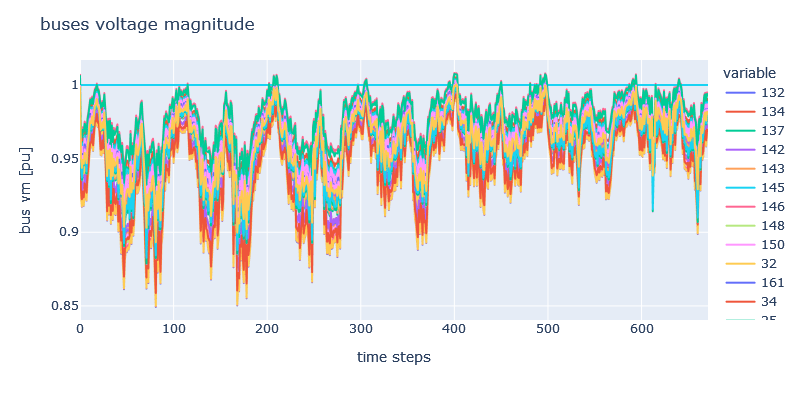
\includegraphics[width=.7\linewidth]{images/MVOberr/High load.png}
% \caption{Case high load. Voltage buses results obtained running the time series}
% \label{fig:gym_anm_net}
% \end{figure}

% In this case, there are only under voltage problems. \\
% The problems are highlighted in the following plot.

% \begin{figure}[h]
% \centering
%     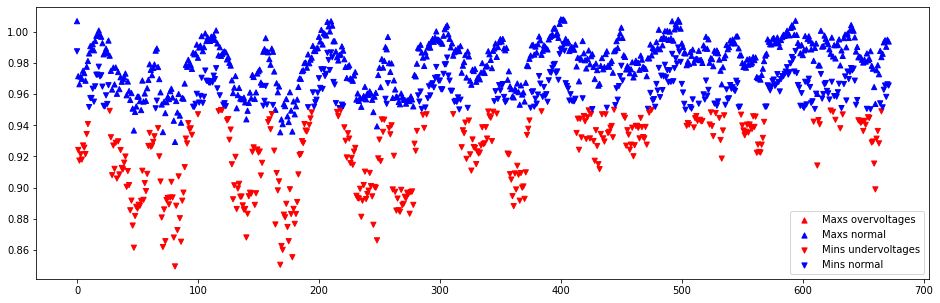
\includegraphics[width=.8\linewidth]{images/MVOberr/High load problems.png}
%     \caption{Same as above, the maximum and minimum values found for each time step and plotted, so for each time step there are two values representing the highest and lowest value among each bus. The colours, blue and red, represent the normal or problem condition.}
% \end{figure}